\documentclass[11pt, a4paper, titlepage, block]{article}
\usepackage{listings}
\hyphenpenalty=10000

\usepackage{graphicx}
\begin{document}
\begin{titlepage}

\newcommand{\HRule}{\rule{\linewidth}{0.5mm}} % Defines a new command for the horizontal lines, change thickness here

\center % Center everything on the page
 
%----------------------------------------------------------------------------------------
%	HEADING SECTIONS
%----------------------------------------------------------------------------------------


%----------------------------------------------------------------------------------------
%	TITLE SECTION
%----------------------------------------------------------------------------------------


%\HRule \\[0.4cm]
{ \huge \bfseries Project Report}\\[1.2cm]
%\HRule \\[0.4cm]

{\LARGE Algoritmi e Strutture Dati}\\[0.5cm]
{\large 2013/2014 summer session}
\\[1.5cm]

{\large Julian Sparber}\\[0.2cm]
{\large matr. no.: 260324}\\[1cm]
%----------------------------------------------------------------------------------------
%	AUTHOR SECTION
%----------------------------------------------------------------------------------------


%----------------------------------------------------------------------------------------
%	DATE SECTION
%----------------------------------------------------------------------------------------

%{\large \today}\\[10cm] % Date, change the \today to a set date if you want to be precise

%----------------------------------------------------------------------------------------
%	LOGO SECTION
%----------------------------------------------------------------------------------------

%\includegraphics{Logo}\\[1cm] % Include a department/university logo - this will require the graphicx package
 
%----------------------------------------------------------------------------------------

\newpage

\end{titlepage}

\section{Specifica del problema}
	Si supponga di elaborare i dati relativi ad un grafo. Le informazioni associate al problema siano: un insieme di vertici (con nomi specifcati da stringhe prive di spazi) e un insieme di archi caratterizzati da una tripla di distanze d1, d2, d3 (una tripla di numeri reali).
	\subsection{}
	Acquisisce da file le informazioni relative al grafo. Il formato del file \`{e} del tipo:\\
	\begin{tabular}{|c|c|c|c|c|}
\hline
	{\textless}No. totale dei vertici{\textgreater} & & & & \\
\hline
	{\textless}No. di vertici collegati al vertice A{\textgreater} & & & & \\
\hline
	{\textless}vertice\_A{\textgreater} & {\textless}vertice\_B{\textgreater} & {\textless}d1{\textgreater} & {\textless}d2{\textgreater} & {\textless}d3{\textgreater}\\
\hline
	{\textless}vertice\_A{\textgreater} & {\textless}vertice\_M{\textgreater} & {\textless}d1{\textgreater} & {\textless}d2{\textgreater} & {\textless}d3{\textgreater}\\
\hline
	... & & & &\\
\hline
	{\textless}vertice\_A{\textgreater} & {\textless}vertice\_Z{\textgreater} & {\textless}d1{\textgreater} & {\textless}d2{\textgreater} & {\textless}d3{\textgreater}\\
\hline
	{\textless}No. di vertici collegati al vertice B{\textgreater} & & & &\\
\hline
	{\textless}vertice\_B{\textgreater} & {\textless}vertice\_C{\textgreater} & {\textless}d1{\textgreater} & {\textless}d2{\textgreater} & {\textless}d3{\textgreater}\\
\hline
	{\textless}vertice\_B{\textgreater} & {\textless}vertice\_X{\textgreater} & {\textless}d1{\textgreater} & {\textless}d2{\textgreater} & {\textless}d3{\textgreater}\\
\hline
	... & & & &\\
\hline
\end{tabular}
Ad esempio:
\begin{lstlisting}
5
3
v_a v_b 8.2 5.3 9.7
v_a v_c 2.5 1.4 3.2
v_a v_e 3.6 5.0 2.7
4
v_b v_a 1.4 5.2 0.1
v_b v_c 8.5 11.4 0.2
v_b v_d 6.0 2.2 2.7
v_b v_e 6.9 2.4 2.8
2
v_c v_d 2.7 6.2 1.1
v_c v_e 3.8 4.4 3.4
3
v_d v_a 18.2 7.3 19.7
v_d v_c 12.5 1.6 5.4
v_d v_e 11.6 3.2 12.7
1
v_e v_a 12.6 16.2 14.1
\end{lstlisting}
	\subsection{}
	Inserisce i dati acquisiti in una opportuna struttura dati.
	\subsection{}
	Dati un vertice sorgente, uno destinazione e una tipologia di distanze (d1 oppure d2 oppure d3) inseriti dall'utente, calcola il percorso pi\`{u} breve tra sorgente e destinazione, mostrando a
monitor tale percorso e la relativa distanza.
	\subsection{}
	Dato un vertice specificato dall'utente, calcola la media e la mediana della distanze minime che separano tale vertice da tutti gli altri vertici del grafo, in base alle tipologie di distanza d1, d2 e d3.\\ \\
	Per quanto riguarda l'analisi teorica si devono studiare le complessit\`{a} degli algoritmi di acquisizione del file (punto 2), calcolo del percorso pi\`{u} breve tra due vertici (punto 3) e calcolo di media e mediana (punto 4).\\
	Per quanto riguarda il punto 4 si deve anche verificare sperimentalmente la complessit\`{a} delcalcolo di media e mediana, generando casualmente una sequenza di distanze (di N numeri reali) da fornire come input all'algoritmo per valori crescenti di N.

	\newpage
\section{Analisi del problema}
	\subsection{INPUT}
		Un vertice sorgente, un vertice destinazione e una tipologia di distanze (d1 oppure d2 oppure d3) viene chiesto all'utente.\\
		Un file sorgete che contine tutte le informazioni sui nodi.\\
	\subsection{OUTPUT}
		All'utente viene mostrato il percorso pi\`{u} breve tra i nodi sorgente e destinazione definiti dall'utente e anche la media e la mediana delle distanze minime dal nodo sorgente a tutti gli altri vertici del grafo.\\
	\subsection{PERCORSO}
	I valori in questo grafo sono distanze qundi non possono essere negativi.
	\subsection{MEDIA}
	La media \`{e} la somma di tutti i valori divsio per il nummero di valori.
	\subsection{MEDIANA}
	La mediana \`{e} il elemento in mezzo di una lista ordinata (o se la lista \`{e} pari la media da i due elementi in mezzo)\\

	\newpage
\section{Progettazione dell'algoritmo}
	Ogni carattere letto dal file viene validato immediatamente. Il nodo e l'arco preso da ognuna delle righe viene salvato in una struttura dinamica di questo tipo: \\\\
	\{\\
	\indent nome del nodo,\\
	\indent archi del nodo,\\
	\indent minima distanza,\\
	\indent parente del nodo,\\
	\indent nodo successivo; \\
	\}\\\\
	e gli archi vengono salvati in una struttura di questo tipo:\\\\
	\{\\
	\indent nome del nodo di destinazione,\\
	\indent nodo di destinazione,\\
	\indent la tripla della distanza,\\
	\indent arco successivo;\\
	\}\\\\

	Visto che i valori in questo grafo sono distanze, non possono essere negativi. Per questa ragione l'algoritmo di Dijkstra \`{e} una buona scelta.\\\\

	La mediana viene calcolata con quickselect, un'algoritmo randomizzato che trova il k-esimo elemento di una struttura disordinata con n elementi eseguendo in O(n$^2$) nel caso pessimo e O(n) nel caso ottimo.\\\\ 

	Quickselect \`{e} relativamente semplice da implementare, e se ben implementato leggermente pi\`{u} veloce di heapselect.\\
	\newpage
\section{Implementazione dell'algoritmo}
	\newpage
\section{Testing del programma}
	\subsection{Output del programma se vengono utilizzato i dati dal esempio}
	\begin{lstlisting}
	Got this Data:
Arcs of: v_a
	v_b with distances: 8.20 5.30 9.70
	v_c with distances: 2.50 1.40 3.20
	v_e with distances: 3.60 5.00 2.70
Arcs of: v_b
	v_a with distances: 1.40 5.20 0.10
	v_c with distances: 8.50 11.40 0.20
	v_d with distances: 6.00 2.20 2.70
	v_e with distances: 6.90 2.40 2.80
Arcs of: v_c
	v_d with distances: 2.70 6.20 1.10
	v_e with distances: 3.80 4.40 3.40
Arcs of: v_d
	v_a with distances: 18.20 7.30 19.70
	v_c with distances: 12.50 1.60 5.40
	v_e with distances: 11.60 3.20 12.70
Arcs of: v_e
	v_a with distances: 12.60 16.20 14.10
Enter the start node
...
	\end{lstlisting}
	\subsection{Output del programma per il percorso da v\_a a v\_b e tipologia 0}
	\begin{lstlisting}
...
Enter the start node
v_a
Enter the end node
v_b
Enter the typology
0
Start and end Node found!
Start routing
The route between v_a and v_b is direct.
The distance between v_a and v_b is 8.200000
Average distance of v_a with all other nodes is: 4.875000
Median distance of v_a with all other nodes is 4.400000
	\end{lstlisting}
	\subsection{Output del programma per il percorso da v\_e a v\_d e tipologia 0}
	\begin{lstlisting}
...
Enter the start node
v_e
Enter the end node
v_d
Enter the typology
0
Start and end Node found!
Start routing
The route between v_e and v_d is
	v_a
	v_c
The distance between v_e and v_d is 17.800000
Average distance of v_e with all other nodes is: 16.575000
Median distance of v_e with all other nodes is 16.450000
	\end{lstlisting}
	\newpage
	\subsection{Output del programma per il percorso da v\_e a v\_d e tipologia 0}
	\begin{lstlisting}
...
Enter the start node
v_e
Enter the end node
v_d
Enter the typology
0
Start and end Node found!
Start routing
The route between v_e and v_d is
	v_a
	v_c
The distance between v_e and v_d is 17.800000
Average distance of v_e with all other nodes is: 16.575000
Median distance of v_e with all other nodes is 16.450000
	\end{lstlisting}
	
		\subsection{Output del programma per il percorso da v\_d a v\_c e tipologia 1}
	\begin{lstlisting}
...
Enter the start node
v_d
Enter the end node
v_c
Enter the typology
1
Start and end Node found!
Start routing
The route between v_d and v_c is direct.
The distance between v_d and v_c is 1.600000
Average distance of v_d with all other nodes is: 6.175000
Median distance of v_d with all other nodes is 5.250000
	\end{lstlisting}
	\newpage
	\subsection{Output del programma per il percorso da v\_a a v\_b e tipologia 2}
	\begin{lstlisting}
...
Enter the start node
v_a
Enter the end node
v_b
Enter the typology
2
Start and end Node found!
Start routing
The route between v_a and v_b is direct.
The distance between v_a and v_b is 9.700000
Average distance of v_a with all other nodes is: 4.975000
Median distance of v_a with all other nodes is 3.750000
	\end{lstlisting}
	\subsection{Output del programma per il percorso da v\_b a v\_a e tipologia 2}
	\begin{lstlisting}
...
Enter the start node
v_b
Enter the end node
v_a
Enter the typology
2
Start and end Node found!
Start routing
The route between v_b and v_a is direct.
The distance between v_b and v_a is 0.100000
Average distance of v_b with all other nodes is: 1.100000
Median distance of v_b with all other nodes is 0.750000
\end{lstlisting}
	
	\newpage
\section{Valutazione della complessit\`{a} del programma}
	Visto che l' algoritmo viene applicato su struttura a grafo, la complessit\`{a} pu\`{o} essere espressa in 
	funzione del numero di vertici e di archi del grafo stesso. A questo scopo verr\`{a} indicato con $|$V$|$ il 
	numero di vertici e con $|$E$|$ (edges) il numero di tutti gli archi.\\
	\\
	La complessit\`{a} dell'algoritmo di acquisizione:\\
	\indent T($|$V$|$, $|$E$|$) = 1+ $|$V$|$ + $|$E$|$ = O($|$V$|$ + $|$E$|$)\\
	La complessit\`{a} dell'algoritmo per calcolare il percorso pi\`{u} breve tra due vertici (Algoritmo di Dijkstra):\\
	\indent T ($|$V$|$, $|$E$|$) = O($|$V$|$ x log $|$V$|$ + $|$E$|$)\\
	La complessit\`{a}  dell'algoritmo per calcolare la media:\\
	\indent T($|$V$|$, $|$E$|$) = O($|$V$|$)\\
	La complessit\`{a} dell'algoritmo per calcolare la mediana (quickselect):\\
	\indent Caso ottimo:\\
	\indent \indent T($|$V$|$, $|$E$|$) = $|$V$|$ + $|$V$|$ + T($|$V$|$ / 2) = O($|$V$|$)\\
	\indent Caso pessimo:\\
	\indent \indent T($|$V$|$, $|$E$|$) = $|$V$|$ + $|$V$|$ + T($|$V$|$ - 1) = O($|$V$|$2)\\
	\newpage
\subsection{Valutazione sperimentale della complessit\`{a} del calcolo di media e mediana}
	Nei risultati della valutazione sperimentale si vede che la complessit\`{a} del calcolo della media \`{e} O($|$V$|$).
	\begin{figure}[htp]
	\centering
	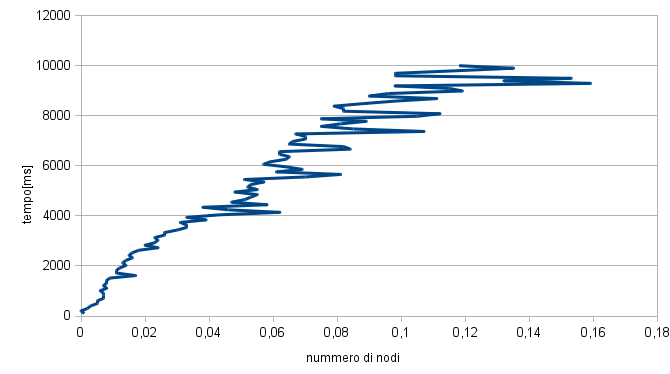
\includegraphics[scale=0.80]{img/calcolo_media.png}
	\caption{complessit\`{a} del calcolo di media}
	\end{figure}
	\newpage
	Anche il risultato dalla valutazione sperimentale del calcolo della mediana non sorprende. Qui si vede il confronto dei calcoli di media e di mediana. 
	La complessit\`{a} varia molto perch\`{e} quickselect \`{e} casuale quindi dipende molto dal vertice di partenza.
	\begin{figure}[htp]
	\centering
	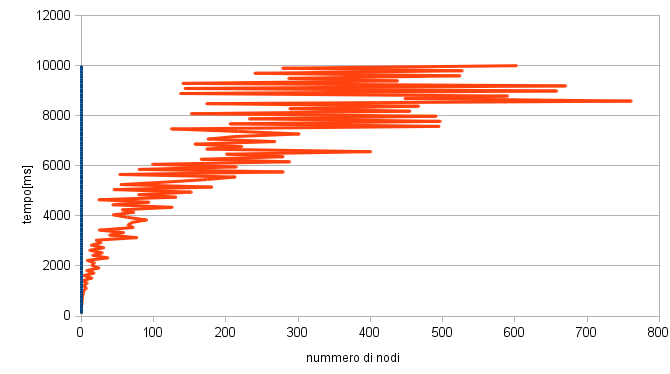
\includegraphics[scale=0.80]{img/calcolo_mediana.png}
	\caption{complessit\`{a} del calcolo di media(blue) e mediana(rosso)}
	\end{figure}

\end{document}
